\documentclass{llncs}

%% Verwende A4-Format statt Letter
\usepackage{a4}
%% Deutsche Silbentrennung und Sprache (neue Rechtschreibung)
%\usepackage[ngerman]{babel}
%% Verwende Schriftart mit "echten" Umlauten statt Akzenten
\usepackage[T1]{fontenc}
%% Verwende Umlaute direkt
\usepackage[utf8x]{inputenc}
%% Hyperlinks für interne Referenzen
\usepackage{hyperref}
%% Grafiken einbinden
\usepackage{graphicx}
%% Paket für Unterabbildungen pro Abbildung
%\usepackage{subfig}

% Titel der Arbeit
\title{Peer-To-Peer in Botnets}

% Angaben zum Author
\author{Moritz Marc Beller}
\institute{%
   Fakultät für Informatik, \\
   Technische Universität München \\
%    Munich, Germany\\
   \email{\{beller\}@in.tum.de}
}

\pagestyle{plain}

%------------------------------------------------------------------------------
\begin{document}

\maketitle

%------------------------------------------------------------------------------
\begin{abstract}
Cyber-attacks are a growing threat to the security of the world. As a
result, in June of 2011, the German government founded a ``national
defense centre against cyber crime''.\cite{cyber} This step became
necessary as new forms of computer worms are no longer restricted to
harming only computers and the data stored on them, as the example of
``Stuxnet'' demonstrates:

 In 2010, a new computer worm called ``Stuxnet'' was discovered. It is
 suspected to have damaged Iran's uranium centrifuges, giving it the
 title ``the first cyber weapon''\cite{benzin2011first}. To spread and
 update, Stuxnet used Internet and Intranet structures to build its
 own {\it botnet}.\cite{fallierew32} Stuxnet is in alignment with a series
 of new botnets using {\it peer-to-peer} communication instead of a
 centralized server. 

This literature review paper focuses on these peer-to-peer botnets and
the growing threat emerging from them. Having read this article, the
reader will be well-informed about current and future techniques in
peer-to-peer botnets.
\end{abstract}

%------------------------------------------------------------------------------
\section{Introduction}

In this work, we describe a new means of communication in botnets,
namely {\it peer-to-peer} communication.  We motivate the research on
botnets by recent real-world examples and introduce common botnet
terminology. We give a classification of P2P botnets and distinguish
different architectures of botnets. In the following sections, we
describe the typical lifetime of a P2P botnet, the command and control
structure in P2P botnets and compare conventional botnets to P2P
botnets. Finally, we described possible countermeasures against P2P
botnets.



\section{Definitions}
A computer able of executing remotely-triggered commands is called a
{\it bot} or {\it zombie.} A {\it botnet} is a group of bots forming a
common network structure.\cite{schoof2007detecting} In most recent
papers on the subject (\cite{wang2009systematic},
\cite{abu2006multifaceted}), the term botnet is defined as purely
negative, i.e. a network performing destructive aims such as
denial-of-service attacks attacks, sending spam or hosting a phishing
website\cite{steggink2007detection}. Other common aims include
providing the aggregated CPU resources of the botnet, stealing user's
credentials \cite{borgaonkar2010analysis} or doing click fraud on
affiliate networks\cite{clickFraud}. Click fraud is the process of
generating clicks on web banners without an actual user seeing or
clicking the advertisment, for the sake of making money. 

In the following, We propose a bias-free definition of botnet as per
our understanding technology is generally ethics-free. Additionally,
there are many examples where botnets are used in a non-destructive
way (e.g. \cite{seti}), or even to destroy existing malicious botnets.

A {\it botmaster} is referred to as the controller of the botnet. This
doesn't necessarily have to be the founder of the botnet (cf. \ref{ClassificP2P}).

The expression {\it bot candidates} specifies the set of computers
which are target to becoming a bot themselves.

{\it P2P}, short for {\it Peer-to-Peer}, being a technology buzz word
of the internet in the late 1990s with the upcoming file sharing
services like Napster\cite{napster}, has attracted less attention in
recent years. P2P defines an unstructured information network
amongst equals --- so-called peers. Two or more peers can
spontaneously exchange information without a central
instance. According to \cite{schoder2005core} ``P2P networks promise
improved scalability, lower cost of ownership, self-organized and
decentralized coordination of previously underused or limited
resources, greater fault tolerance, and better support for building ad
hoc networks.''  These properties coupled with the fact that files
exchanged in P2P networks are prone to malware, trojans and viruses
make P2P networks a most-attractive base for building botnets. With so many 
Well-known P2P networks include the Napster\cite{napster}, Gnutella,
Overnet and Torrent network.  A {\it P2P bot} then is a bot that uses
a P2P protocol as a means of communication with other bots.

The so-called {\it C\&C}, command and control structure, specifies
the way and protocols in which the botmaster and the bots communicate
with each other. It is the central property of any botnet. Common
protocols for C\&C include IRC, HTTP, FTP and
P2P.\cite{borgaonkar2010analysis}

{\it IRC} --- internet relay chat --- is a ``teleconferencing
system''\cite{irc}, typically used for text chatting in channels
joined by a large number of participants. While its protocol is
relatively easy to implement, it provides a lot of features. It has
thus become the one of the most widely-used protocols for C\&C in
conventional botnets.

The process of {\it bootstrapping} generally describes starting a more
complex system outof a simple system. In regard to botnets, the
term usually means loading of the bot code (often injected into the
original filesharing program) and establishing a connection to other
bots.\cite{wang2009systematic}

\section{A brief history of botnets}
The origins for the term ``bot'' go back to so-called IRC bots, short
for IRC robots. An IRC bot is a program that handles specific tasks in
the IRC automatically, so that the administrator does not need to do
those routine jobs.

The first IRC bot ever to be created was named Eggdrop. Its origins go
back to the year 1993. However, in April 1998 a deriviant called
GT-Bot appeared and formed the first malicious botnet, using IRC's
C\&C structures. Four years later, in 2002, Slapper was the first
botnet to make use of P2P for C\&C.\cite{li2009botnet}

\section{The genesis of a P2P botnet}


\subsection{Classification P2P networks}
\label{ClassificP2P}
There are three types of P2P networks: ``parasite'', ``leeching'' and
``bot-only''.\cite{wang2009systematic} 

Parasite and leeching bots infiltrate existing P2P networks, while
``bot-only'' networks are designed as new networks. 

Parasite botnets recruit new bots only from the set of existing P2P
participants; they try to infect system inside the P2P network and
make them become bots. Due to the often illegal content distributed in
file sharing networks, they are a perfect culture medium of viruses,
malware and worms. It is thus convenient for an attacker to spread a
highly-demanded file (e.g. some cracked computer game, software or
porn) containing the injection code sequences for his bot. This code is
then injected into the file sharing client. Vulnerable hosts in the
network are infected this way. On the downside, this means that the
spread of the bot is limited to the size of the P2P network.

In contrast, leeching bots not only try to infiltrate systems which
are already part of the P2P network, but also systems outside of the
P2P network. Natuarally, they are bigger in size as they have to
deliver the P2P client, too. This might be more difficult to achieve
as it means that systems must unwillingly take part in the
network. Often, firewalls and port-forwarding are not configured for
use with the P2P network on these systems, reducing the performance of
the botnet: Since the owner of the computer usually doesn't even know
he is participating in a P2P network, he has no intention of opening
the ports in his firewall. Leeching bots can spread through any
possible measure: File sharing, downloads on websites, email
attachments and instant messanging.

There are good reasons for either strategy: Using an existing P2P
network as a base --- like parasite and leeching bots do --- unburdens
the botmaster from setting up and building a botnet infrastructure. It
profits from the established P2P network, making use of filtering,
error-correction and encryption as far as the chosen network has
support for it. On the other hand, features are limited to the
existing P2P protocol. A specifically-built P2P bot-only network is
natuarally more tailored towards its purpose. Due to the bot-exclusive
memberships, it might be easier to shutdown the botnet for an attacker
as all participants can be considered bots and there is no risk of
accidentally shutting down an innocent member. Bot-only networks are
described in detail in \ref{decent}.


\subsection{Lifetime of P2P botnets}
Wang et al.\cite{wang2009systematic} differentiate three stages of P2P botnets:
\begin{itemize}
\item Recruiting bot members (infecting others)
\item Forming the botnet (construction phase)
\item Standing by for instruction \\
This is the actual ``operational'' phase of the botnet. Bots are awaiting instructions from their master. Instructions can either be actual commands or performing updates. In this phase, the chosen C\&C structure is essential.
\end{itemize}
It should be noted that these phases are not strictly exclusive,
e.g. during the third phase (standing by for instruction), building of
the botnet may well continue. In fact, this is an inherent property of
any P2P network: Constant transformation of the network. It is only
until a critical mass of bots has proceeded past phase one and two,
that the botnet can be called operational.

\section{Architectures of Botnets}
In reality, there exist two principally different architectures of
botnets. A new architecture has been proposed by scientists, which
combines the advantages of both. The following nomenclature is
extracted from \cite{steggink2007detection}:
\subsection{Centralized Architecture}
%
% Das Bild aus Buch soundso von Seite soundso
%
\begin{figure}[htbp]
  \centering
  \fbox{
    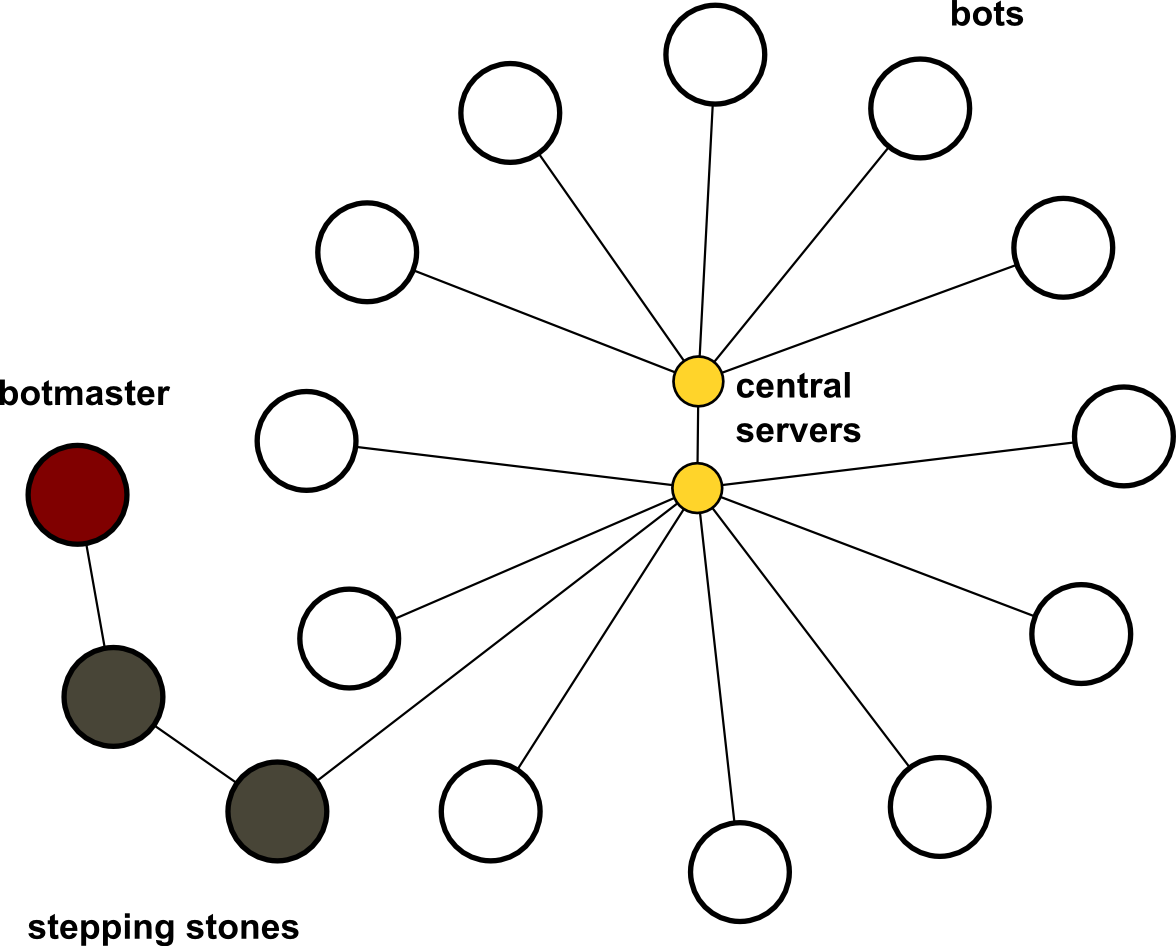
\includegraphics[width=0.8\textwidth]{figures/central-network.png}
  }
  \caption{Graph depicting connections in a centralized network. Note
    how all bots only have a connection to the central point. (Source: Own work)}
  \label{central-network}
\end{figure}
Historically the oldest form of botnets, centralized architectures are
built up in such a way that there is one central spot which broadcasts
messages between the connected bots and the botmaster.  It's common to
have more than one central server\cite{td1sc}, but even with several
servers, the architecture still stays centralized. For if you shutdown
this central point, the network is inoperable. This resembles the
biggest weakness of centralized architectures: As soon as you are able
to cut the server off the net, the network is dead. On the other hand,
latency becomes minimal, as the routing distance for one package
needed to reach each node in the network is minimal (only one
transition is needed). Bandwidth, however, is generally limited by the
server's resources, making it hard to receive or transmit big chunks
of data. Furthermore, it holds that all the routes in the network have
the same length. This is something which is fundamentally more complex
in decentralized networks and can be a great simplification of command
distribution and monitoring the network.

Due to their nature, centralized architectures are usually implemented
with an IRC C\&C or similar\cite{cooke2005zombie}. The central server
is normally not owned by the botmaster. This would make detecting his
identity easy. In many countries, launching an ``evil-minded botnet''
is a serious crime. Instead, hacked or public IRC servers are used as
the central C\&C node. A connection from the attacker's computer to
the central server is often obfuscated by many in-between relays,
tunnels and encryption. In figure
\ref{central-network} this is shown as the ``steeping stones'' which
shall hide an attacker's idenity.

 A criminal conviction because of launching a botnet is thus
 relatively seldom. Yet, in 2007, John Schiefer was sentenced to four
 years in prison. He built a botnet with up to 250,000 zombies,
 collecting passwords and bank credentials from the bots.\cite{BotnetCrime}

\subsection{Decentralized Architecture}
\label{decent}
Dezentralized architectures do not rely on the special role of one
central server. Instead, they are built upon the principal of
equality, namely that the ``peer nodes (both client and server) are
all equal''\cite{steggink2007detection}. The topology of the network
is far more complex than in centralized architectures, forming a mesh
as shown in figure \ref{p2p-network}. It is thus more difficult for a
bot to join the botnet. Extensive bootstrapping is required, as the
bot has to figure out an already-participating peer to connect to in the
beginning. Once inside the net, information about other peers is
exchanged between nodes. There are two approaches for bootstrapping\cite{wang2009systematic}:
\begin{itemize}
\item A list of peers likely to be online is hardcoded into the client. This list can later be updated
\item A shared web cache on the internet stores information about
  peers. The address of which is hardcoded.
\end{itemize}

As can be seen, Bootstrapping is a critical and vulnerable point in
any P2P botnet. Considerable efforts by botmaster have been made to
circumvent the need to bootstrap\cite{td1sc}. This is further
discussed in \ref{counter-measure}.

Once inside the net, information about other peers is
exchanged between nodes.

Distributing commands and data in such a network is complicated, as it
has to be assured that the message reaches all clients. As a general
rule of thumb, the better inter-connected the nodes are, the higher
the probability for a message to reach all recipients.

A decentralized network has the advantage of having the accumulated
resources and bandwidth of all the peers in the network
available. However, latency might be bad, as routing through the
network is not trivial (cf. figure \ref{p2p-network}). P2P networks
are generally considerd to be harder to disable (cf. section
\ref{counter-measure} on page \pageref{counter-measure}).

It is to be discussed whether P2P networks with a centralized server
architecture for certain services like file-indexing --- we refer to
them as ``Napster-like'' botnets --- fall into the ``decentralized''
category. Principally, the connection graph differs a lot from
centralized networks, but centralized and Napster-like networks share
the same weaknesses, as could be seen when Napster was shut down in
2001\cite{napsterWiki}.\footnote{This was performed as an act of
  cofirming with the decision made in the intellectual property case
  of US A&M Records, Inc. v. Napster, Inc., 239 F.3d 1004 (2001) and
  not an explicit attack against the Napster network, but the fact
  that the Napster network could so easily stop the network by just
  disconnecting its central server shows the inherent weakness of
  centralized architectures.}  Dittrich et
al. \cite{dittrich2007command} would consider Napster-like botnets a
hybrid architecture, whereas Steggink et al.
\cite{steggink2007detection} classify it as decentralized. In the
following, we stick with Steggink's definition, as there seems to be a
broader consensus in the literature towards their nomenclature
(cf. \cite{td1sc}).

% P2P network picture
\begin{figure}[htbp]
  \centering
  \fbox{
    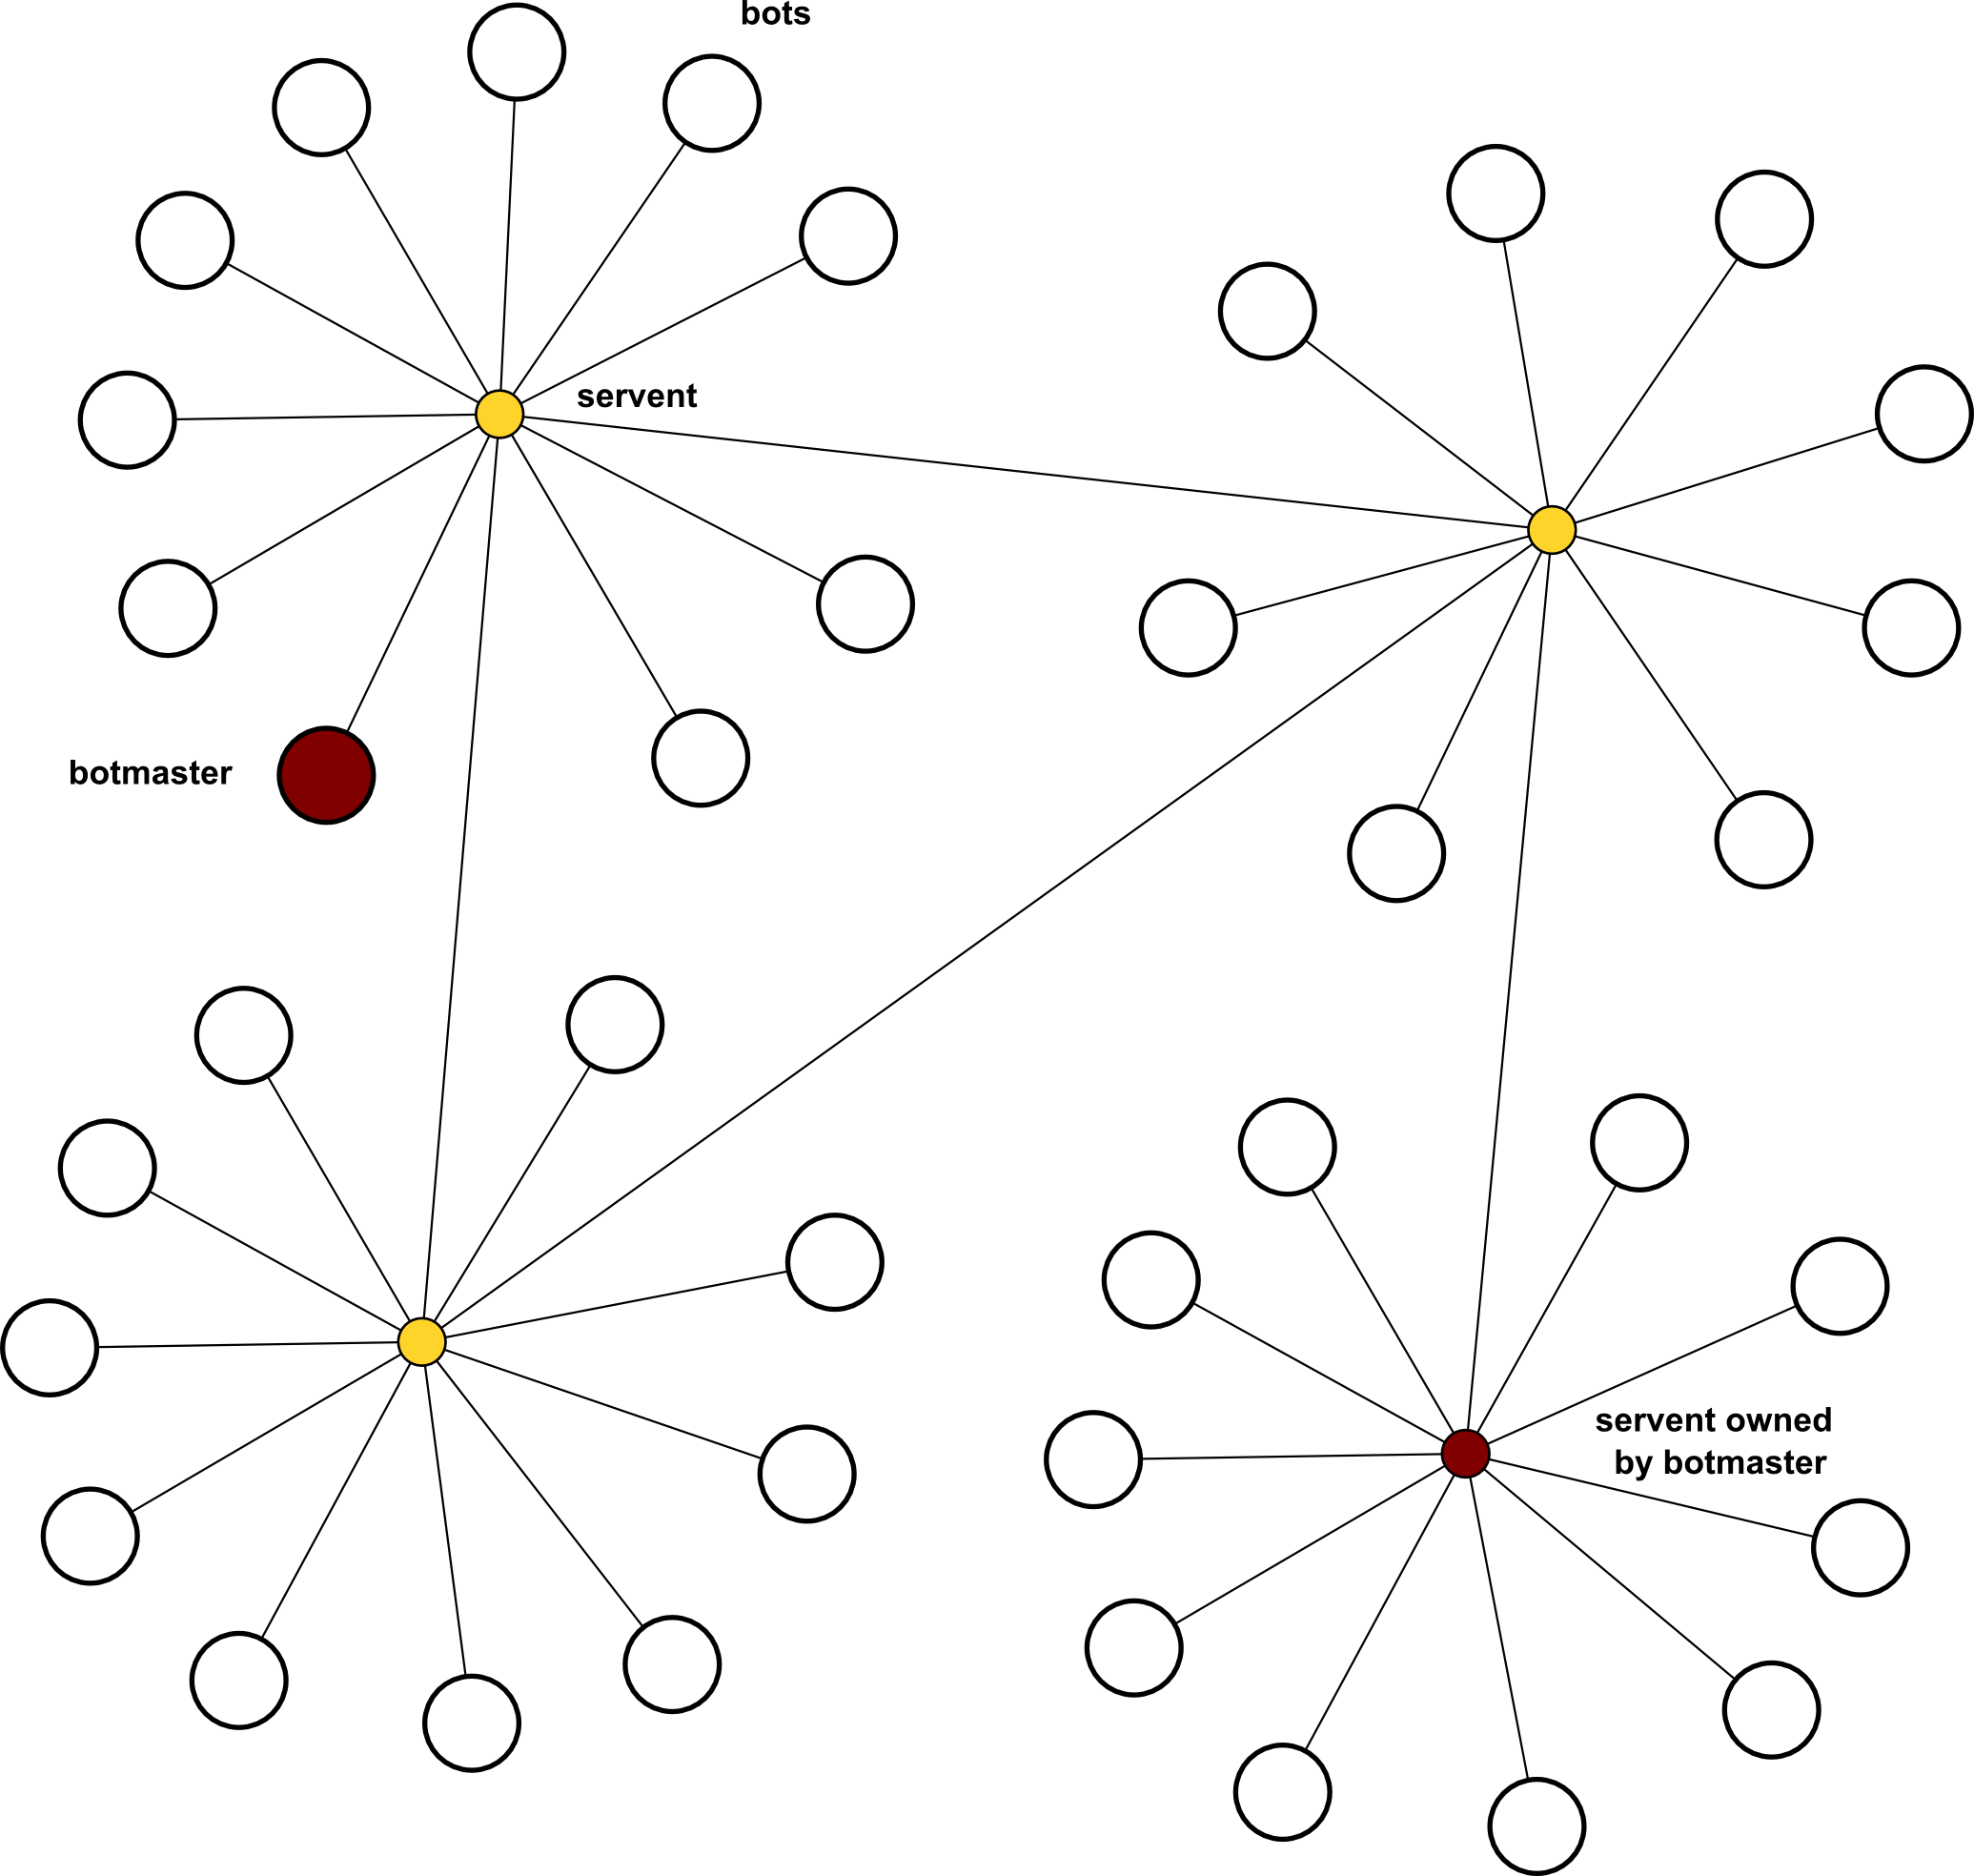
\includegraphics[width=0.7\textwidth]{figures/p2p-network.png}
  }
  \caption{P2P network (Source: \cite{dittrich2007command})}
  \label{p2p-network}
\end{figure}


\subsection{Hybrid Architecture}
Hybrid architectures are botnet architectures driven by scientific
development and up to this date only exist in theory. They have been
described as ``the advanced P2P botnet''\cite{td1sc} and the ``super
botnet''\cite{vogt2007army}. The approach is to study current botnets,
analyze their weaknesses and propose a better solution. This
anticipates how botmasters could improve their botnets in the
future. This way, even today, we know what future botnets could look
like and how to better defend against them.

The proposed new hybrid P2P botnets do not have a pre-set
communication architecture, following the strict P2P definiton. Their
network connectivity is solely determined by the {\it peer list} in
each bot.

Only machines with static IPs appear as bots in the peer list,
so-called {\it servents}.'\cite{td1sc} This way, it is guranteed that
the distributed peer lists are maximally deadlink-free.  This is a
specialization of the ``all peers are equal'' contract in P2P: Some
bots --- the servents --- have special obligations described in the
following.  The clients are then typically bots behind firewalls,
machines with private or dynamic IPs.

\subsubsection{Network construction phase}

Infection is done no different than in conventional botnets
(cf. \ref{ClassificP2P}). The basic construction procedure has two
mechanisms:
\begin{itemize}
\item {\bf New Infection:} ``Bot A passes its peer list to a
vulnerable host B when compromising it. If A is a
servent bot, B adds A into its peer list (by randomly
replacing one entry if its peer list is full). If A knows
that B is a servent bot (A may not be aware of
B’s identity, for example, when B is compromised by
an e-mail virus sent from A), A adds B into its peer
list in the same way.'' \cite{td1sc}
\item {\bf Reinfection:} ``If bot A
reinfects bot B, bot B will then replace \lbrack{}a series of\rbrack{} 
 randomly selected bots in its peer list with \lbrack{}...\rbrack{} bots
from the peer list provided by A. Again, bots A and B
will add each other into their respective peer lists if
the other one is a servent bot.''\cite{td1sc}
\end{itemize}

Both the advanced P2P botnet and the super botnet have their own P2P
protocols for C\&C. They implement push and pull
C\&C.\cite{wang2009systematic} When a bot receives a command it
forwards it to all the peers in its list (push). If a bot cannot
accept incoming connections (due to network misconfiguration, or a
firewall), it actively polls other peers in its connection list from
time to time to receive new commands (pull, cf. \ref{pushpull} on page
\pageref{pushpull}).

\subsubsection{Lifetime Comparison against superbot net}

In the following, we will concentrate on the ``the advanced P2P
botnet'' as described by \cite{td1sc}. It was shown by Wang et
al. \cite{td1sc} that the super botnet suggested by Vogt et al. is not
likely to become successful in a real world scenario:

% distribution graph picture
\begin{figure}[htbp]
  \centering
  
    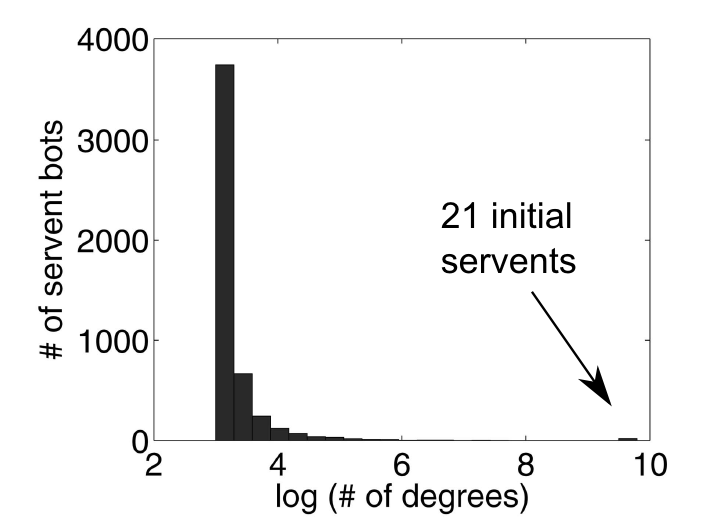
\includegraphics[width=0.6\textwidth]{figures/distributiongraph.png}
  
  \caption{Degree-distribution graph of servent bots assuming only new-infections and reinfections (derived work, original source: \cite{td1sc}). Simulation constraints: possible vulnerable hosts $n=500,000$, stop of growth of botnet after $n=20,000$, peer list size $M=20$, 21 initial servent bots.}
  \label{distributiongraph}
\end{figure}

% distribution graph picture
\begin{figure}[htbp]
  \centering
  
    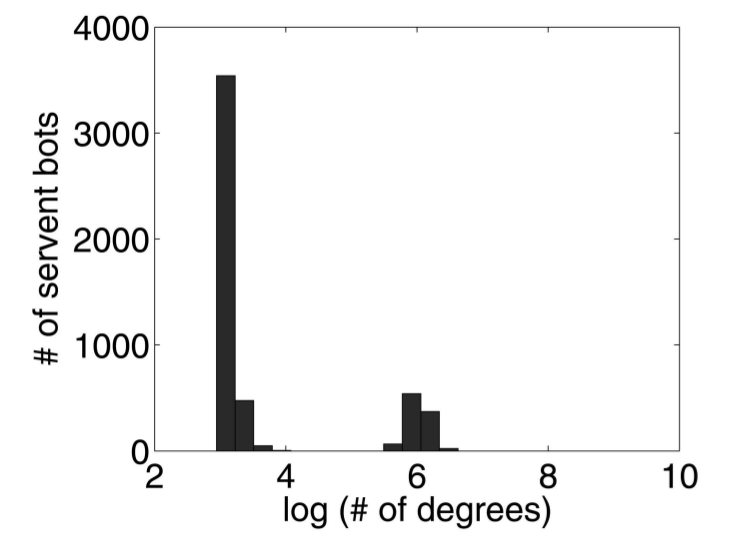
\includegraphics[width=0.6\textwidth]{figures/distributiongraph2.png}
  
  \caption{Degree-distribution graph of servent bots simulating peer list update propagation, also (Source: \cite{td1sc}). Most notably, the 21 initial servent bots cannot be spotted. Instead, a robust backbone for the P2P network has formed out of 1,000 servent bots $v$ (around x-axis 6), $deg(v) \in [300;500]$.}
  \label{distributiongraph2}
\end{figure}

\begin{itemize}
\item \label{nat} In contrast to what Vogt et al. assume, most of the
  compromised computers cannot act as servents (due to a firewall,
  NAT\footnote{Network Address Translation, occurs behind a router}
  or dynamic IP address) in the real world.
\item Even though Vogt et al. demonstrated the robustness of their
  constructed botnet (cf. \cite{vogt2007army}), they rely on the
  assumption that enough reinfections will occcrr during the early
  lifetime of the botnet, namely the buildup-phase. According to
  \cite{td1sc} this is a false assumption as heavy reinfection-seeking
  during buildup will lead to easy detection of the botnet and a lot
  of wasted resources. Following this approach, Wang et al. showed
  that the super botnet algorithms for propagation --- namely only
  ``new infection'' and ``reinfection'' --- require over 200,000
  infections events to create an evenly balanced botnet of only 20,000
  vulnerable bots. As a result, when not enough reinfections occur, a
  scenario as depicted in figure \ref{distributiongraph} arises:
  Because the botnet stops growth after having infected 20,000 hosts,
  but there is such a huge amount of vulnerable hosts (500,000), a
  reinfection event rarely ever happens. This means that servent bots
  only seldom exchange parts of their peer lists. As a consequence,
  the connection to servent bots is extremely unbalanced: In the
  network graph, 80\% of servent bots have a degree less than 30,
  while the initial 21 servents have degrees between 14,000 -- 17,000:
  Most of the newly introduced servents have very few peers (both
  clients and servents) connected to them, essentially degrading the
  P2P botnet to a central network with 21 main servers. This is by no
  means an ideal P2P botnet.

When it is not possible to have enough reinfections, the ``new
infection'' and ``reinfection'' propagation measures are obviously not
enough.
\end{itemize}

\subsubsection{Peer list updating}
Because of this problem, Wang et al. propose a new, third propagation
method: Peer list updating. The idea behind this is that bots update
their peer lists frequently. However, this imposes a severe security
problem: An attacker capturing only one bot could soon reveal the
identity of many servents in the network. Thus, a new command is
introduced: Enforced peer list updating. As described in \cite{td1sc},
it is possible for a botmaster to monitor his botnet, i.e. determine
how many servents exist. After a sufficiently large time after
construction phase, he can enforce a peer list update: All bots obtain
a new peer list from a specified {\it sensor host}. This sensor host
is equipped with the knowledge of all the servents in the network by
the monitor-command issued by the botmaster. Upon query, the sensor
host creates a peer list in the following way: It randomly chooses
servent bots, composes an updated peer list out of them and sends it
back to the querying bot. After each peer list update command, all
bots will have ``uniform and balanced connections.''\cite{td1sc}

The network graph obtained is then similar to the one shown in figure
\ref{p2p-network} on page \pageref{p2p-network}.

It is to be discussed at which point in time it makes sense for the
botmaster to enforce a peer list update, for every update command
bears the risk of discovery of parts of the network. This is further
discussed in \cite{td1sc}. Simulations with an update after the first
1,000 infections show that this update strategy will result in a
degree distribution depicted in figure \ref{distributiongraph2}: The
first 1,000 servents have many balanced connections ($deg(v) \in
[300;500]$), forming the robust backbone and connecting the hybrid P2P
network tightly together. However, the remaining 4,000 servents
(connected to the network after the update-command was run) have the
known symptom of having degrees between 20-30, a situation well-known
from the simulations of the superbot net (cf. figure
\ref{distributiongraph}). Thus, a forced peer list update from time to
time seems necessary to make for a good P2P infrastructure.

\begin{figure}[htbp]
  \centering
  \fbox{
    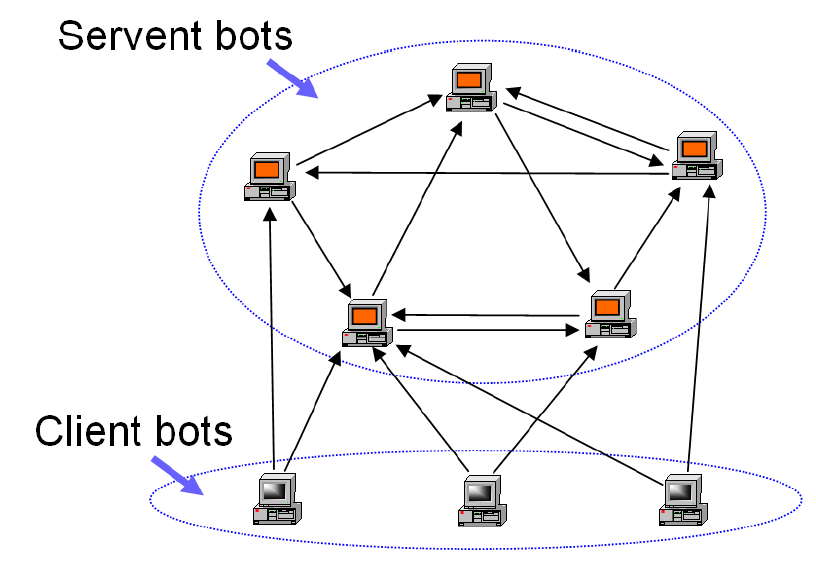
\includegraphics[width=0.7\textwidth]{figures/hybrid-network.png}
  }
  \caption{Hybrid network (Source: \cite{td1sc})}
  \label{hybrid-network}
\end{figure}

\subsubsection{Further improvements}

The proposed hybrid network has several other advantages over common,
existing P2P networks: It doesn't need bootstrapping, removing a
single point of failure. Bootstrapping is avoided due to the three
propagation measures (new infections, reinfections and forced peer
list updates). An initial peer list is simply passed on to the newly
infected zombie by the machine infecting it. Due to its fixed size
peer list ($M=20$ in the simulations for \ref{distributiongraph},
\ref{distributiongraph2}), when an attacker gets access to a bot, it
doesn't reveal whole (sub-)nets.  Only machines with static IPs appear
as peer bots, so-called {\it servents}. This way, it is guranteed that
the distributed peer lists are maximally deadlink-free. Data
encryption in the hybrid P2P botnet has two functions: First, it makes
it hard to sniff for patterns in internet traffic to detect a possible
botnet. Second, the authenticity of the issued commands can be
verified so that only commands signed by the botmaster are
executed. The bot software can be shipped with a hardcoded public key
from the botmaster.

\begin{figure}[htbp]
  \centering
  \fbox{
    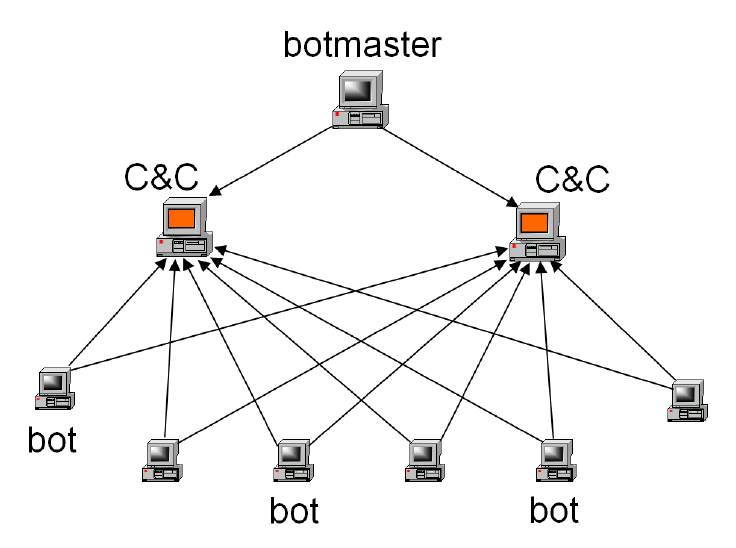
\includegraphics[width=0.7\textwidth]{figures/central-network2.png}
  }
  \caption{Another graphical representation of a central network (Source: \cite{td1sc})}
  \label{central-network2}
\end{figure}

Compared to a central-strucutre botnet (see \ref{central-network2}),
the hybrid P2P net (see \ref{hybrid-network}) is only an extension of the
orginial network: It is essentially equivalent to a central
architecture P2P net. However, the amount of servers (in the form of
servents) is greatly increased, as is the number of interconnections
between them. The great number of servents is the primary reason why
the hybrid P2P botnet is supposedly very hard to shut
down.\cite{td1sc}

As tempting as such an advanced new botnet protocol may sound, it has
to be acknowedlged that the hybrid P2P botnet is a purely academical,
theoretical idea that has never been tested in practice: ``The network
may not be as stable and robust as expected due to complex network
conditions and defenses.''\cite{wang2009systematic}

\section{Command and Control structures in P2P botnets}
Central server, hybrid, completely decentralized

Dezentralized: Peacom p.7 in 10.1.1.112.3561.pdf
see p. 3 in 10.1.1.153.8296

authentication of commands

\subsection{Push/Pull mechanism}
\label{pushpull}
Commands can be distributed in two ways: Either via a push or a pull mechanism. ``Pulling'', being the more trivial of the two approaches, is the process of a client actively asking a server whether there's new instructions for it. To be up-to-date this has to be perforemd periodically, increasing network load.
Push on the other hand is technically more advanced, as commands from the server will be automatically ``pushed'' to the clients --- the difference between push and pull in a bot is much like IMAP IDLE compared to POP3 for mail: With POP3, the user client has to periodically ask the server whether there are new messages available (pull), whereas with IMAP, the client gets a new message pushed by the server. This has the advantage of reducing the network traffic, but it requires that the server can open a connection to the clients (cf. \ref{nat}). 

\section{Comparison: Conventional bots vs. P2P bots}
some real world examples of P2P bots and what their c\&c etc. looks like
tbw.

\section{Detection of and Counter measure against evil P2P botnets}
\label{counter-measure}
What can an attacker do to de-arm a botnet at all? The ideal solution would be to shutdown all participants in the botnet (and only those). Realistically, this is almost never possible. It is also illegal in most countries to start a botnet, as it implies gaining access to another computer. This falls into the category of hacking. On the other hand, paradoxically, shutting down a botnet is likewise illegal, for it requires the attacker --- be he benign or not --- to do the same: Hacking into computers. Sub-tasks in fighting a botnet are therefore:
\begin{itemize}
\item Detecting the botnet at all
\item Analyzing the botnet: Finding servers, zombies, estimating the size of the botnet
\item Preventing further spread of botnet: Fixing security exploit of injection vector
\item Disabling the bot(sub-)nets: Making clients loose inter-connection, shutting down central servers
\item Infiltrating botnet to do non-malicious tasks
\end{itemize}

While it is --- in theory --- realtivley easy to shutdown a centralized architecture by determining the central servers and disabling those (e.g. through DoS attacks\footnote{Denial of Service attacks, i.e. generating so much traffic the target cannot function normally any more}), P2P networks are arguably harder to disable, given they are properly protected. 

\subsection{Index-poisoning}
Napster-like P2P networks use an index to determine where to get a
certain file from. 

<-- insert more detailed description of p2p indices -->

``Originally, index poisoning attack was introduced to prevent
illegal distribution of copyrighted content in P2P networks. The main
idea is to insert massive number of bogus records into the index. If a
peer receives bogus record, it could end up not being able to locate
the file (nonexistent location), or downloading the wrong
file''\cite{wang2009systematic}

Once you know under which keys the botnet commands are stored in the
index records, an attacker trying to shutdown the network can insert
false commands under the same keys. If there is enough false
information, chances to hit the real command issued by the botmaster
are slim. The index gets ``flooded'' or poisned by wrong
commands. These can either be NOPs (no operations, meaning a command
that does nothing), or may even help to disguise the botnet.

Index-poising has been reported to have succeeded
in fighting two recent P2P bots, namely Trojan.Peacomm and
Stormnet. (\cite{grizzard2007peer}, \cite{liang2006index})


\subsection{Sybil attack}

\subsection{Bootstrapping}
Bootstrapping is a vulnerable point in any P2P botnet. When a
hardcoded peer list is used (cf. \ref{decent} for details), it is
sufficient to take down all the peers in the bootstrapping table for
the network to eventually shutdown: New bots simply can't find an
initial peer to connect to. Botmasters have reacted to this by
providing a Gnutella-like web-cache or updateable bootstrapping
tables.

%------------------------------------------------------------------------------
\bibliographystyle{alpha}
\bibliography{literature}



\end{document}
